\chapter{Juegos en Forma Extensiva}
\label{chapter:juegos-forma-extensiva}

Muchos juegos constan de una secuencia de acciones realizadas por los jugadores a lo largo del tiempo, haciendo al modelo anterior insatisfactorio debido a que ignora la estructura secuencial de este tipo de problemas de decisión. Estos juegos pueden ser representados en forma de árbol enraizado, donde cada nodo representa un estado del juego y las ramas representan las acciones que se pueden realizar en un nodo (o estado) específico. 

\begin{example}[{\cite[p. 91]{bib:course-game-theory}}]
\label{ex:game-allocation}
Dos personas utilizan el siguiente procedimiento para compartir dos objetos idénticos e indivisibles. Una de ellas propone una asignación, que la otra persona acepta (A) o rechaza (R). Si la propuesta es aceptada se lleva a cabo dicha división. En caso de rechazo, ninguna persona recibe ninguno de los dos objetos. Cada persona sólo se preocupa sobre la cantidad de objetos que tiene. 
\end{example}

La Figura \ref{fig:game-allocation} representa el árbol correspondiente al juego presentado. Cada nodo representa un estado del juego. Los nodos no terminales tienen un jugador asignado, que representa quien debe tomar la decisión en ese estado y las ramas representan las acciones posibles. En este caso la raíz corresponde al primer jugador, el cual tiene $3$ opciones posibles: quedarse con los $2$ objetos: $(2-0)$, repartir $1$ objeto para cada jugador: $(1-1)$, o darle los $2$ objetos al jugador $2$: $(0-2)$. Los $3$ nodos del primer nivel corresponden al jugador $2$, en cada uno de ellos tiene dos opciones: aceptar o rechazar la distribución. Las hojas representan los nodos terminales del juego, cada uno con la ganancia respectiva para cada jugador según el caso.

\begin{figure}[h]
\begin{center}
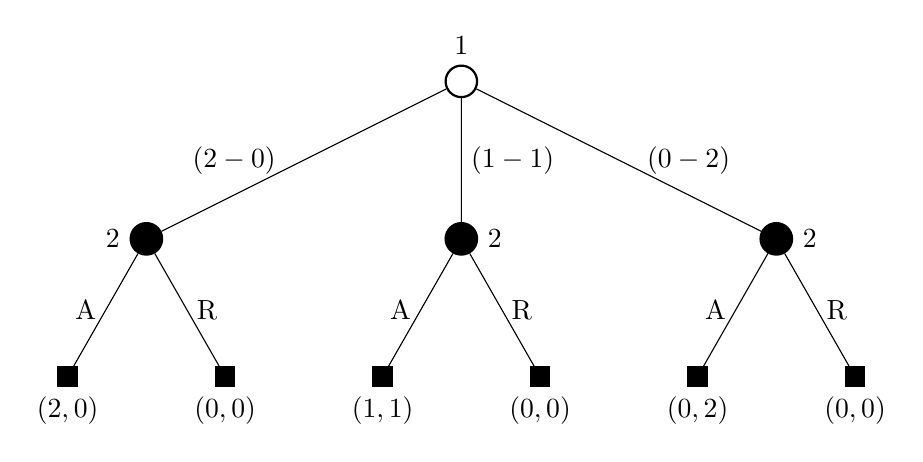
\begin{tikzpicture}[
player1/.style={circle, draw=black, thick, minimum size = 4mm},
player2/.style={circle, draw=black, fill=black, thick, minimum size=4mm},
terminal/.style={rectangle, draw=black, fill=black, thick, minimum size=2mm},
level 1/.style={sibling distance=40mm, level distance=20mm},
level 2/.style={sibling distance=20mm, level distance=17.5mm},
]
\node[player1] [label=$1$]{}
    child { node [player2] [label=left:{$2$}] {}
    	child { node [terminal] [label=below:{$(2,0)$}] {}
        		edge from parent node[left] {A} }
        child { node [terminal] [label=below:{$(0,0)$}] {}
        		edge from parent node[right] {R} }
        edge from parent node[left] {$(2-0)\ \ $}
    }
    child { node [player2] [label=right:{$2$}] {}
    	child { node [terminal] [label=below:{$(1,1)$}] {}
        		edge from parent node[left] {A} }
        child { node [terminal] [label=below:{$(0,0)$}] {}
        		edge from parent node[right] {R} }
        edge from parent node[right] {$(1-1)$}
    }
    child { node [player2] [label=right:{$2$}] {}
    	child { node [terminal] [label=below:{$(0,2)$}] {}
        		edge from parent node[left] {A} }
        child { node [terminal] [label=below:{$(0,0)$}] {}
        		edge from parent node[right] {R} }
        edge from parent node[right] {$\ \ (0-2)$}
    };
\end{tikzpicture}
\caption{Árbol del juego en forma extensiva del Ejemplo~\ref{ex:game-allocation}. Los nodos del primer jugador son representados con círculos sin relleno, los nodos del segundo jugador con círculos con relleno negro y los nodos terminales con cuadrados con relleno negro.}
\label{fig:game-allocation}
\end{center}
\end{figure}

Es importante diferenciar entre dos tipos de juegos: con información completa (o perfecta) y con información incompleta (o imperfecta). En los juegos con información completa los jugadores tienen toda la información sobre las acciones realizadas previamente de todos los jugadores y del estado actual del juego. El Ejemplo \ref{ex:game-allocation} es un ejemplo de este tipo de juegos; para una definición formal ver \cite[pp. 89--90]{bib:course-game-theory}.

En juegos con información incompleta el jugador no tiene toda la información de las acciones tomadas previamente, e incluso pudo haber olvidado las acciones que él u otro jugador realizaron previamente. Por lo cual, un jugador puede no tener suficiente información para determinar en qué nodo del árbol se encuentra. 

\begin{example}[{\cite[p.~202]{bib:course-game-theory}}]
\label{ex:informacion-incompleta}
Considere un juego de dos jugadores, el jugador $1$ y el jugador $2$, el cual ocurre como sigue: primero, el jugador $1$ debe elegir una opción entre $L$ y $R$. Si elige $R$ el juego termina; si elige $L$ se le informa al jugador $2$ que el jugador $1$ eligió $L$ y este debe elegir una opción entre $A$ y $B$. Por último, el jugador $1$ debe escoger una nueva opción entre $l$ y $r$, pero sin saber que opción eligió el jugador $2$. Los pagos son mostrados en las hojas del árbol del juego, presentado en la Figura~\ref{fig:informacion-incompleta}.
\end{example}

\begin{figure}[h]
\begin{center}
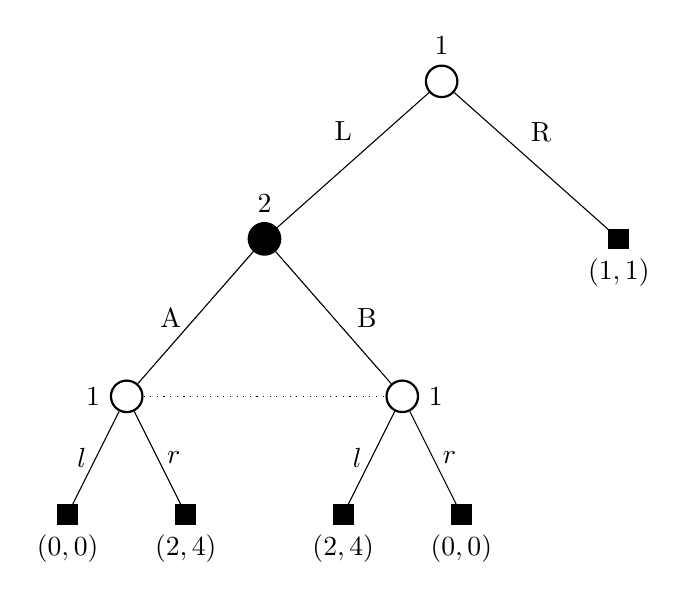
\begin{tikzpicture}[
player1/.style={circle, draw=black, thick, minimum size = 4mm},
player2/.style={circle, draw=black, fill=black, thick, minimum size=4mm},
terminal/.style={rectangle, draw=black, fill=black, thick, minimum size=2mm},
level 1/.style={sibling distance=45mm, level distance=20mm},
level 2/.style={sibling distance=35mm, level distance=20mm},
level 3/.style={sibling distance=15mm, level distance=15mm},
]
\node[player1] [label=$1$] {}
	child { node [player2] [label=above:{$2$}]  {}
    	child { node (A) [player1] [label=left:{$1$}]  {} 
        		child { node [terminal] [label=below:{$(0,0)$}] {} 
                		edge from parent node[left] {$l$} }
                child { node [terminal] [label=below:{$(2,4)$}] {}
                		edge from parent node[right] {$r$}}
                edge from parent node[left] {A\, }
        }
        child { node (B) [player1] [label=right:{$1$}] {}
        		child { node [terminal] [label=below:{$(2,4)$}] {}
                		edge from parent node[left] {$l$} }
                child { node [terminal] [label=below:{$(0,0)$}] {} 
                		edge from parent node[right] {$r$} }
                edge from parent node[right] {\, B}
        }
        edge from parent node[left] [label=above:{L}] {}
    }
    child { node [terminal] [label=below:{$(1,1)$}] {}
    		edge from parent node[right] [label=above:{R}] {}
    };
\draw[dotted] (A) -- (B);
\end{tikzpicture}
\caption{Árbol del juego en forma extensiva presentado en el Ejemplo~\ref{ex:informacion-incompleta}. Los nodos que pertenecen al mismo conjunto de información son unidos por líneas punteadas.}
\label{fig:informacion-incompleta}
\end{center}
\end{figure}

Se puede observar que los nodos unidos por líneas punteadas son indistinguibles para el jugador $1$, pues él no sabe cuál fue la elección del jugador $2$. Este tipo de nodos originan los llamados \textbf{conjuntos de información}; cf.\ Definición~\ref{def:informacion-incompleta} y \cite[p.~200]{bib:course-game-theory}. El concepto de conjunto de información es intrínseco a los juegos en forma extensiva y no es necesario para juegos en forma normal. Se asumirá que los conjuntos de información vienen definidos de forma explícita en el modelo de juego en forma extensiva; una definición basada en el árbol del juego puede ser encontrada en \cite{bib:conceptos-basicos}.

\begin{definition}
\label{def:informacion-incompleta}
Un juego finito en \textbf{forma extensiva} con \textbf{información incompleta} tiene los siguientes componentes:
\begin{itemize}[]
  \item Un conjunto finito $N$ de \textbf{jugadores}.
  \item Un conjunto finito $H$ de secuencias, las posible \textbf{historias} de acciones, tal que la secuencia vacía está en $H$, y cada prefijo de una secuencia en $H$ también está en $H$. $Z \subseteq H$ son las historias terminales (aquellas que no son prefijo de ninguna otra secuencia). $A(h) = \{ a : (h, a) \in H \}$ son las acciones disponibles después de una historia no terminal $h \in H$. Si la historia $h$ es prefijo de la historia $h'$ escribimos $h\sqsubseteq h'$, y si $h$ es un prefijo propio de $h'$ escribimos $h\sqsubset h'$.
  \item Una función $P$ que asigna a cada historia no terminal (cada elemento de $H \setminus Z)$ un elemento de $N \cup \{c \}$. $P$ es la \textbf{función de jugador}. $P(h)$ es el jugador que toma una acción después de la historia $h$. Si $P(h) = c$ entonces la acción tomada después de la historia $h$ es determinada por el azar. Este tipo de nodos serán denominados \textbf{nodos de azar}.
  \item Una función $f_c$ que asocia con cada historia $h$, para la cual $P(h) = c$, una medida de probabilidad $f_c(\cdot|h)$ sobre $A(h)$: $f_c(a|h)$ es la probabilidad de que la acción $a$ ocurra dado $h$.  Cada medida de probabilidad es independiente de cualquier otra de estas medidas.
  \item Para cada jugador $i \in N$, una partición $\mathcal{I}_i$ de $\{h \in H : P(h) = i\}$ con la propiedad de que $A(h) = A(h')$ siempre que $h$ y $h'$ estén en el mismo bloque de la partición. Para $I_i \in \mathcal{I}_i$ se denota por $A(I_i)$ el conjunto $A(h)$ y por $P(I_i)$ el jugador $P(h)$ para cualquier $h \in I_i$. $\mathcal{I}_i$ es la \textbf{partición de información} del jugador $i$, un conjunto $I_i \in \mathcal{I}_i$ es un \textbf{conjunto de información} del jugador $i$.
  \item Para cada jugador $i \in N$, una función de utilidad $u_i$ de los estados terminales $Z$ a los reales $\mathbb{R}$. Si $N = \{1,2\}$ y $u_1 = -u_2$, se dice que se tiene un \textbf{juego de dos jugadores de suma cero en forma extensiva}. Se define $\Delta_{u,i} = \max_z u_i(z) - \min_z u_i(z)$ como el rango de utilidades del jugador $i$.
\end{itemize}
\end{definition}

En el Ejemplo \ref{ex:informacion-incompleta}, $H = \{ \emptyset, L, R, LA, LB, LAl, LAr, LBl, LBr\}$, note que la cantidad de elementos en $H$ coincide con la cantidad de nodos del árbol. En efecto, en un árbol para cualquier nodo $u$ existe un camino único desde la raíz hasta $u$. Además, $P(\emptyset) = P(LA) = P(LB) = 1$, y $P(L) = 2$ indican a cuál jugador le toca jugar en cada nodo del árbol. Las particiones de información son $\mathcal{I}_1 = \{\{\emptyset\}, \{LA, LB\}\}$ y $\mathcal{I}_2  = \{\{L\}\}$. En la definición se incluye un elemento que no está presente en el ejemplo, los \textbf{nodos de azar}. Estos nodos corresponden a acciones que no dependen de los jugadores, sino de algún evento externo aleatorio, como el lanzamiento de una moneda, lanzamiento de uno o más dados, o la repartición de cartas en un juego.

\subsection*{Juego de Kuhn Poker}
\label{section:kuhn-poker}

Kuhn Poker es una versión simplificada del juego de Póker con tres cartas y dos jugadores (denominados jugador $1$ y jugador $2$) definido por Harold W.\ Kuhn \cite{bib:kuhn-poker}. En este juego se barajan tres cartas marcadas con los números $1$, $2$ y $3$. Posteriormente, cada jugador recibe una de ellas, manteniendo su número como información privada. Es decir, un jugador sabe su propio número pero no sabe el número de su oponente. Al inicio del juego cada jugador apuesta una ficha. El juego ocurre por turnos, los cuales se alternan entre los jugadores comenzando por el jugador $1$. En un turno un jugador puede \textit{apostar} o \textit{pasar}. Si un jugador apuesta debe apostar una ficha adicional. Si un jugador pasa después de una apuesta, el oponente gana y toma todas las fichas apostadas. Si hay dos apuestas o dos pases seguidos los jugadores muestran sus cartas y gana el jugador con el número más alto obteniendo todas las fichas apostadas. La Tabla \ref{table:kuhn-poker} presenta un resumen de todas las posibles secuencias con su respectivo pago a cada jugador.

\begin{table}[h]
\begin{center}
\caption[Resumen de las posibles secuencias del juego Kuhn Póker]{Resumen de las posibles secuencias del juego Kuhn Póker.}
\label{table:kuhn-poker}
\begin{tabular}{ c c c c }
\toprule
\multicolumn{3}{c}{Secuencia de Acciones} & \multirow{2}{*}{Pago} \\ \cmidrule{1-3}
Jugador $1$ & Jugador $2$ & Jugador $1$ &  \\ \midrule
\multirow{3}{*}{pasar} & pasar & & $+1$ al jugador con la carta más alta\\
& apostar & pasar & $+1$ al jugador $2$\\
& apostar & apostar & $+2$ al jugador con la carta más alta \\ \midrule
\multirow{2}{*}{apostar} & pasar & & $+1$ al jugador $1$ \\
& apostar & &  $+2$ al jugador con la carta más alta \\ \bottomrule
\end{tabular}
\end{center}
\end{table}

Debido a qué es un juego de suma $0$, el jugador perdedor pierde el número de fichas que gana su oponente. El árbol del juego se muestra en la Figura \ref{fig:kuhn-poker}. La raíz es un \textit{nodo de azar}, que representa la repartición de las cartas, con $6$ opciones diferentes, las cuales están representadas con un par ordenado indicando la carta del jugador $1$ y la del jugador $2$. Cada rama tiene una probabilidad de $\frac{1}{6}$ de ser elegida. Los nodos del primer nivel y tercer nivel corresponden al jugador $1$. Este jugador tiene $6$ conjuntos de información diferentes, cada uno con $2$ nodos, los cuales se unen mediante las líneas punteadas. Los nodos del segundo nivel corresponden al jugador $2$, los conjuntos de información se representan por nodos del mismo color y mismo estilo (relleno de color o no). En cada nodo de decisión (los nodos no terminales sin incluir la raíz), hay dos opciones: pasar, representado con una línea discontinua, o apostar, representado con una línea doble. Los nodos terminales tienen la ganancia del jugador $1$, según sea el caso.

\begin{figure}[h]
\begin{center}
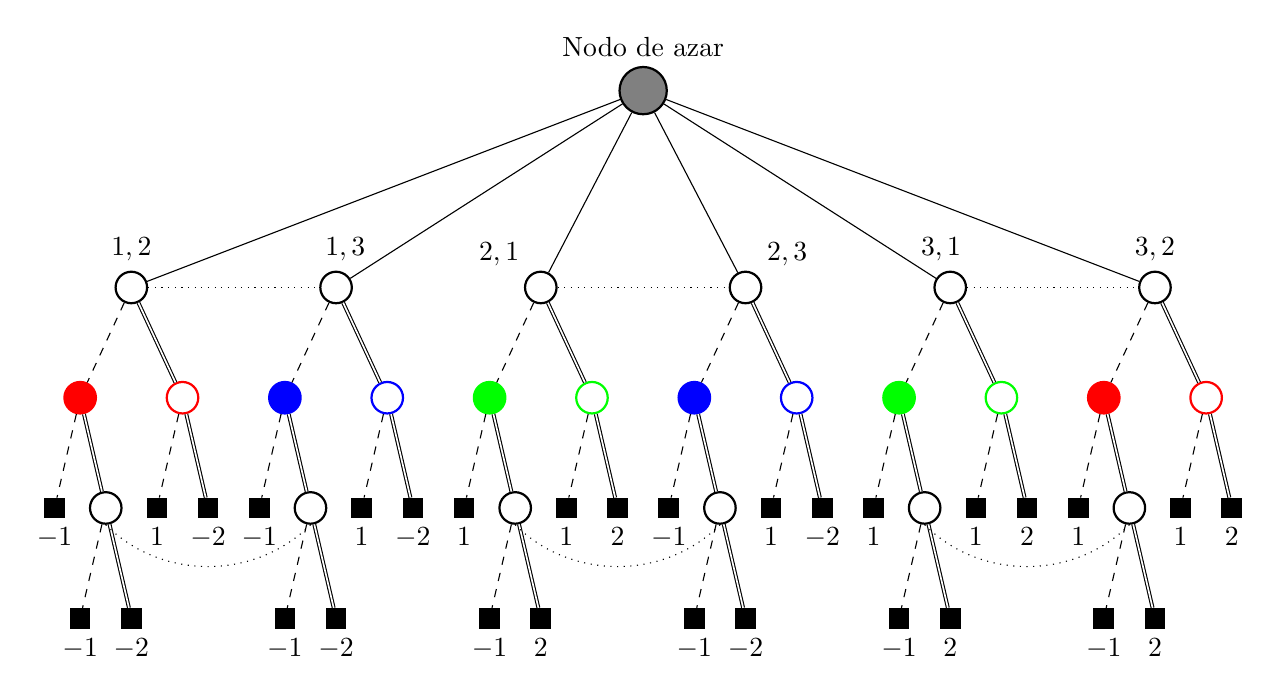
\begin{tikzpicture}[
chance/.style={circle, draw=black, fill=gray, thick, minimum size = 6mm},
player1/.style={circle, draw=black, solid, thick, minimum size = 4mm},
player2/.style={circle, thick, minimum size=4mm},
terminal/.style={rectangle, draw=black, solid, fill=black, thick, minimum size=2mm},
level 1/.style={sibling distance=26mm, level distance=25mm},
level 2/.style={sibling distance=13mm, level distance=14mm},
level 3/.style={sibling distance=6.5mm, level distance=14mm},
]
\node[chance] [label=above:{Nodo de azar}] {} {
	child {node [player1] (P1) [label=above:{$1, 2$}]{}
		child { node [player2] [draw=red, fill=red] {} 
				child { node [terminal] [label=below:{$-1$}] {}
						edge from parent [dashed] {} }
				child { node [player1] (A) {} 
						child { node [terminal] [label=below:{$-1$}] {}
								edge from parent [dashed] {} }
						child { node [terminal] [label=below:{$-2$}] {} 
								edge from parent [solid, double] {} }
						edge from parent [solid, double] {}
				}
				edge from parent [dashed] {}
		}
		child { node [player2] [draw=red] {} 
				child { node [terminal] [label=below:{$1$}] {}
						edge from parent [dashed] {} }
				child { node [terminal] [label=below:{$-2$}] {}
						edge from parent [solid, double] {} }
				edge from parent [solid, double] {}
		}
	}
	child {node [player1] (P2) [label=above:{$\ \ 1, 3$}]{}
		child { node [player2] [draw=blue, fill=blue] {} 
				child { node [terminal] [label=below:{$-1$}] {}
						edge from parent [dashed] {} }
				child { node [player1] (B) {} 
						child { node [terminal] [label=below:{$-1$}] {}
								edge from parent [dashed] {} }
						child { node [terminal] [label=below:{$-2$}] {}
								edge from parent [solid, double] {} }
						edge from parent [solid, double] {}
				}
				edge from parent [dashed] {}
		}
		child { node [player2] [draw=blue] {} 
				child { node [terminal] [label=below:{$1$}] {}
						edge from parent [dashed] {} }
				child { node [terminal] [label=below:{$-2$}] {}
						edge from parent [solid, double] {} }
				edge from parent [solid, double] {}
		}
	}
	child {node [player1] (P3) [label=135:{$2, 1$}]{}
		child { node [player2] [draw=green, fill=green] {} 
				child { node [terminal] [label=below:{$1$}] {}
						edge from parent [dashed] {} }
				child { node [player1] (C) {} 
						child { node [terminal] [label=below:{$-1$}] {}
								edge from parent [dashed] {} }
						child { node [terminal] [label=below:{$2$}] {}
								edge from parent [solid, double] {} }
						edge from parent [solid, double] {}
				}
				edge from parent [dashed] {}
		}
		child { node [player2] [draw=green] {} 
				child { node [terminal] [label=below:{$1$}] {}
						edge from parent [dashed] {} }
				child { node [terminal] [label=below:{$2$}] {}
						edge from parent [solid, double] {} }
				edge from parent [solid, double] {}
		}
	}
	child {node [player1] (P4) [label=45:{$2, 3$}]{}
		child { node [player2] [draw=blue, fill=blue]{} 
				child { node [terminal] [label=below:{$-1$}] {}
						edge from parent [dashed] {} }
				child { node [player1] (D) {} 
						child { node [terminal] [label=below:{$-1$}] {}
								edge from parent  [dashed] {} }
						child { node [terminal] [label=below:{$-2$}] {}
								edge from parent [solid, double] {} }
						edge from parent [solid, double] {}
				}
				edge from parent [dashed] {}
		}
		child { node [player2] [draw=blue] {} 
				child { node [terminal] [label=below:{$1$}] {}
						edge from parent [dashed] {} }
				child { node [terminal] [label=below:{$-2$}] {}
						edge from parent [solid, double] {} }
				edge from parent [solid, double] {}
		}
	}
	child {node [player1] (P5) [label=above:{$3, 1\ \ $}]{}
		child { node [player2] [draw=green, fill=green] {} 
				child { node [terminal] [label=below:{$1$}] {}
						edge from parent [dashed] {} }
				child { node [player1] (E) {} 
						child { node [terminal] [label=below:{$-1$}] {}
								edge from parent [dashed] {} }
						child { node [terminal] [label=below:{$2$}] {}
								edge from parent [solid, double] {} }
						edge from parent [solid, double] {}
				}
				edge from parent [dashed] {}
		}
		child { node [player2] [draw=green] {} 
				child { node [terminal] [label=below:{$1$}] {}
						edge from parent [dashed] {} }
				child { node [terminal] [label=below:{$2$}] {}
						edge from parent [solid, double] {} }
				edge from parent [solid, double] {}
		}
	}
	child {node [player1] (P6) [label=above:{$3, 2$}]{}
		child { node [player2]  [draw=red, fill=red] {} 
				child { node [terminal] [label=below:{$1$}] {}
						edge from parent [dashed] {} }
				child { node [player1] (F) {} 
						child { node [terminal] [label=below:{$-1$}] {}
								edge from parent [dashed] {}}
						child { node [terminal] [label=below:{$2$}] {}
								edge from parent [solid, double] {} }
						edge from parent [solid, double] {}
				}
				edge from parent [dashed] {}
		}
		child { node [player2]  [draw=red] {} 
				child { node [terminal] [label=below:{$1$}] {}
						edge from parent [dashed] {} }
				child { node [terminal] [label=below:{$2$}] {}
						edge from parent [solid, double] {} }
				edge from parent [solid, double] {}
		}
	}
};
\draw[dotted]
(A.south) .. controls ++(-45:10mm) and ++(45:-10mm) .. (B.south);
\draw[dotted]
(C.south) .. controls ++(-45:10mm) and ++(45:-10mm) .. (D.south);
\draw[dotted]
(E.south) .. controls ++(-45:10mm) and ++(45:-10mm) .. (F.south);
\draw[dotted] (P1.east) -- (P2.west);
\draw[dotted] (P3.east) -- (P4.west);
\draw[dotted] (P5.east) -- (P6.west);
\end{tikzpicture}
\end{center}
\caption{Árbol completo del juego Kuhn Póker. Los nodos unidos con líneas punteadas o con el mismo diseño y color pertenecen a el mismo conjunto de información. En cada nodo de decisión la acción \textit{pasar} es representada con una línea discontinua y la acción \textit{apostar} es representada con una línea doble.}
\label{fig:kuhn-poker}
\end{figure}

\section{Estrategias Puras y Mixtas para Juegos en Forma Extensiva}

Al igual que en juegos en forma normal es necesario establecer las definiciones de estrategias. Las Definiciones \ref{def:estrategia-pura-fe} y \ref{def:estrategia-mixta-fe}, presentan los conceptos de estrategia pura y estrategia mixta, análogas a las presentadas en los juegos en forma normal. Las definiciones de perfiles estratégicos son equivalentes a las anteriores pero usando los conceptos de estrategias para juegos en forma extensiva. Además, se procura utilizar una notación similar a la utilizada en la sección anterior. Sin embargo, se presenta un nuevo concepto, las \textbf{estrategias de comportamiento}, que son exclusivas para juegos en forma extensiva. A continuación, se sigue la formulación de \cite{bib:conceptos-basicos} y \cite{bib:course-game-theory}.

\begin{definition}
\label{def:estrategia-pura-fe}
Una \textbf{estrategia pura} para el jugador $i$ es una función $s_i : \mathcal{I}_i \rightarrow \bigcup_{I_i \in \mathcal{I}_i}A(I_i)$ tal que $s_i(I_i) \in A(I_i)$, donde $A(I_i) = A(h)$ para cualquier $h \in I_i$ es el conjunto de acciones permitidas después de la historia $h$. 
\end{definition}

Note que una estrategia pura consiste en elegir una acción por cada conjunto de información de un jugador en específico. Considere nuevamente el Ejemplo \ref{ex:informacion-incompleta}. En este juego el jugador $1$ tiene dos conjuntos de información, $I^1 = \{\emptyset\}$ e $I^2 = \{LA, LB\}$, cada uno con dos posibles elecciones, dando lugar a $4$ estrategias puras que son denotadas por $s_1$, $s_2$, $s_3$ y $s_4$, y mostradas en la Tabla~\ref{table:estrategias-puras}. En dicha tabla las acciones posibles en el conjunto de información $I^1$ están representadas por las filas, y las acciones en $I^2$ por las columnas. De esta forma cada celda representa una única estrategia pura determinada por una acción en cada conjunto de información.

\begin{table}[h]
\begin{center}
\caption{Estrategias puras para el juego con información incompleta presentado en el Ejemplo \ref{ex:informacion-incompleta}.}
\label{table:estrategias-puras}
\begin{tabular}{c c | c | c | }
 \multicolumn{2}{c}{} & \multicolumn{2}{c}{$I_2$} \\
 \multicolumn{2}{c}{} & \multicolumn{1}{c}{l} & \multicolumn{1}{c}{r} \\ \cline{3-4}
 \multirow{2}{*}{$I_1$} & $L$ & $s_1=$  elegir L y l & $s_2=$ elegir L y r\\ \cline{3-4}
 & $R$ & $s_3=$ elegir R y l & $s_4=$ elegir R y r \\ \cline{3-4}
\end{tabular}
\end{center}
\end{table}

En Kuhn Póker una estrategia pura para el jugador $2$ puede ser la siguiente: si su carta contiene el número $1$ siempre pasa, si su carta contiene el número $2$ apuesta si y sólo si el jugador $1$ pasa en su primer turno, y si su carta contiene el número $3$ siempre apuesta. La Tabla \ref{table:ejemplo-estrategia-pura} presenta cada conjunto de información de forma explícita con su acción correspondiente. Para este juego se caracterizarán los conjuntos de información del jugador $2$ por la carta que tiene y la acción realizada por el primer jugador al inicio del juego.

\begin{table}[h]
\begin{center}
\caption{Ejemplo de una estrategia pura para el jugador $2$ en el juego Kuhn Poker.}
\label{table:ejemplo-estrategia-pura}
\begin{tabular}{ c c c }
\toprule
\multicolumn{2}{c }{Conjunto de Información} & \multirow{2}{*}{Acción del jugador $2$} \\ \cmidrule(r){1-2}
Carta del jugador $2$ & Acción del jugador $1$ &  \\ \midrule
$1$ & pasar & pasar \\
$1$ & apostar & pasar \\
$2$ & pasar & apostar \\
$2$ & apostar & pasar \\
$3$ & pasar & apostar \\
$3$ & apostar & apostar \\
\bottomrule
\end{tabular}
\end{center}
\end{table}

Se denotará, al igual que en los juegos en forma normal, con $S_i$ al conjunto de estrategias puras del jugador $i$, es decir $S_i=\prod_{I_i \in \mathcal{I}_i} A(I_i)$. Análogamente, se denotará con $S = \prod_{i \in N} S_i$ el conjunto de todas las estrategias puras de todos los jugadores de forma simultánea. Un elemento $s \in S$ es llamado un \textbf{perfil estratégico}.

Otra definición de interés es la función de pago para una estrategia pura. Para esto se denotará con $\pi^s(h)$ la probabilidad de que $h \in H $ ocurra si todos los jugadores juegan con la estrategia $s$. Luego, se define $u_i : S \rightarrow \mathbb{R}$ como la esperanza de la función de pago para el jugador $i$ para cada perfil estratégico, la cual viene dada por:
\begin{alignat}{1}
\label{eq:funcion-pago-fe}
u_i(s)\ =\ \sum_{z \in Z} \pi^s(z) u_i(z) \,.
\end{alignat} 

\begin{definition}
\label{def:estrategia-mixta-fe}
Una \textbf{estrategia mixta} $\sigma^m_i$ para el jugador $i$ es una distribución de probabilidad sobre $S_i$. Es decir, $\sigma_i^m \in \Delta(S_i)$.
\end{definition}

\begin{definition}
Un \textbf{perfil estratégico mixto} $\sigma^m \in \prod_{i \in N} \Delta(S_i)$ consiste en una estrategia mixta para cada jugador de forma $\sigma^m = (\sigma_1^m, \sigma_2^m, ...., \sigma_N^m)$.
\end{definition}

Un perfil estratégico mixto indica que cada jugador elige, \emph{antes de que el juego comience}, un plan completo (es decir, una estrategia pura) de forma aleatoria acorde a cierta distribución de probabilidad (que está dada por su estrategia mixta respectiva).

Si $\sigma^m \in \prod_{i = 1}^N \Delta(S_i)$ es un perfil estratégico mixto, la ganancia esperada del jugador $i$, cuando todos los jugadores juegan acorde a $\sigma^m$ viene dada por:
\begin{alignat}{1}
u_i(\sigma^m)\ =\ \sum_{s \in S} \sigma^m(s)u_i(s)
\end{alignat}
donde $\sigma^m(s)$ es la probabilidad de que $s$ sea elegida, es decir $\sigma^m(s) = \prod_{i \in N} \sigma_i^m(s_i)$.

\section{Forma Normal vs. Forma Extensiva}
\label{section:normal-extensiva}

Un juego en forma normal se caracteriza por el conjunto de estrategias puras $S_i$ y la función de pago $u_i$ para cada jugador $i\in N$. Estos elementos pueden obtenerse a partir de la descripción de un juego en forma extensiva utilizando las definiciones \ref{def:estrategia-pura-fe} y \ref{eq:funcion-pago-fe}. De esta forma, es posible asociar un único juego en forma normal a cualquier juego en forma extensiva.

En el Ejemplo \ref{ex:informacion-incompleta}, las estrategias puras para el jugador $1$ están definidas en la Tabla \ref{table:estrategias-puras}. El jugador dos tiene sólo dos estrategias puras, elegir $A$ o $B$. Luego, la Tabla \ref{table:fextensiva-a-fnormal} es la tabla de pagos para juego en forma normal que corresponde al Ejemplo \ref{ex:informacion-incompleta}.

\begin{table}[h]
\begin{center}
\caption[Forma normal de un juego en forma extensiva]{Tabla de pagos de la forma normal correspondiente a la forma extensiva del juego presentado en el Ejemplo \ref{ex:informacion-incompleta}.}
\label{table:fextensiva-a-fnormal}
\begin{tabular}{c c|c|c|}
\multicolumn{2}{c}{} & \multicolumn{2}{c}{Jugador $2$} \\ 
\multicolumn{2}{c}{} & \multicolumn{1}{c}{Elegir $A$} & \multicolumn{1}{c}{Elegir $B$} \\ \cline{3-4}
\multirow{4}{*}{Jugador $1$} & Elegir $L$ y $l$ & $0,0$ & $2,4$ \\ \cline{3-4}
& Elegir $L$ y $r$ & $2,4$ & $0,0$ \\ \cline{3-4}
& Elegir $R$ y $l$ & $1,1$ & $1,1$ \\ \cline{3-4}
& Elegir $R$ y $r$ & $1,1$ & $1,1$ \\ \cline{3-4}
\end{tabular}
\end{center}
\end{table}

Note que la tabla obtenida tiene $8$ configuraciones a pesar que el árbol original tiene únicamente $5$ nodos terminales. En general, la forma normal tiene un tamaño exponencial en el tamaño del árbol del juego en forma extensiva. Se observa que más de una celda (o una estrategia pura) lleva al mismo nodo terminal. Esto ocurre cuando el primer jugador elige $R$, en este caso no importa las elecciones posteriores pues el juego termina inmediatamente. Por esto la forma normal de un juego es potencialmente más grande que su forma extensiva.

Por otra parte, dado un juego en forma normal, siempre es posible construir el árbol de una forma extensiva como sigue \cite{bib:conceptos-basicos}: se comienza por la raíz, la cual es el único nodo del jugador $1$, de ésta salen $|S_1|$ ramas, una para cada estrategia pura $s_1 \in S_1$, estos nodos, los hijos de la raíz, serán los nodos del jugador $2$. De cada uno de los nodos del jugador $2$ salen $|S_2|$ ramas, una por cada elemento $s_2 \in S_2$ que serán los hijos del jugador $3$, y así sucesivamente hasta llegar a los hijos de los nodos del jugador $N$, que serán los nodos terminales. La Figura \ref{fig:RPS}, muestra el árbol para una forma extensiva del juego piedra (R), papel (P) o tijera (S).

\begin{figure}[h]
\begin{center}
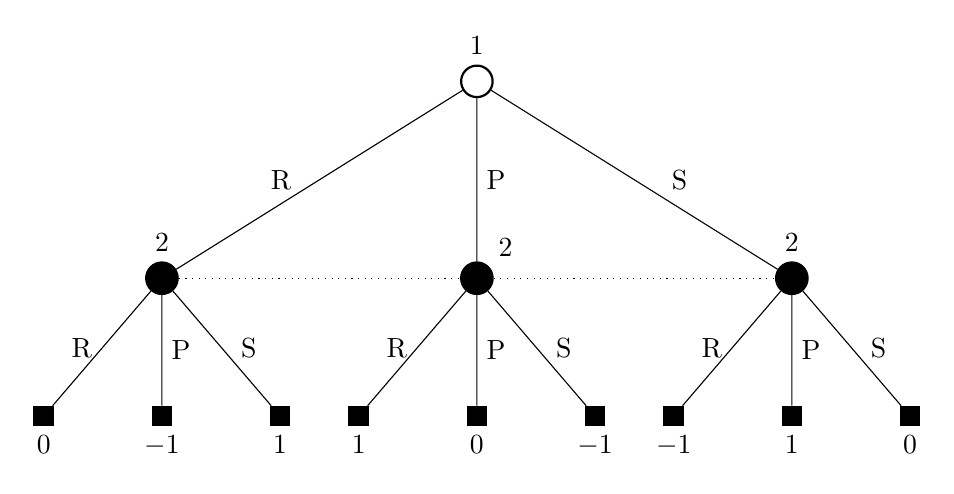
\begin{tikzpicture}[
chance/.style={circle, draw=black, fill=black, thick, minimum size = 6mm},
player1/.style={circle, draw=black, thick, minimum size = 4mm},
player2/.style={circle, draw=black, fill=black, thick, minimum size=4mm},
terminal/.style={rectangle, draw=black, fill=black, thick, minimum size=2mm},
level 1/.style={sibling distance=40mm, level distance=25mm},
level 2/.style={sibling distance=15mm, level distance=17.5mm},
]
\node[player1] [label=$1$] {}
	child { node (A) [player2] [label=above:{$2$}]  {}
    	child { node [terminal] [label=below:{$0$}] {}
        		edge from parent node[left] {R\ } }
        child { node [terminal] [label=below:{$-1$}] {}
        		edge from parent node[right] {P} }
        child { node [terminal] [label=below:{$1$}] {}
        		edge from parent node[right] {\ S} }
    edge from parent node[left] {R\ \ \ }
    }
    child { node (B) [player2] [label=45:{$2$}] {}
    	child { node [terminal] [label=below:{$1$}] {}
        		edge from parent node[left] {R\ } }
        child { node [terminal] [label=below:{$0$}] {}
        		edge from parent node[right] {P} }
        child { node [terminal] [label=below:{$-1$}] {}
        		edge from parent node[right] {\ S} }
    edge from parent node[right] {P}
    }
    child { node (C) [player2] [label=above:{$2$}] {}
    	child { node [terminal] [label=below:{$-1$}] {}
        		edge from parent node[left] {R\ } }
        child { node [terminal] [label=below:{$1$}] {}
        		edge from parent node[right] {P} }
        child { node [terminal] [label=below:{$0$}] {}
        		edge from parent node[right] {\ S} }
    edge from parent node[right] {\ \ \ S}
    };
\draw[dotted] (A) -- (B) -- (C);
\end{tikzpicture}
\caption{Árbol de la forma extensiva del juego piedra, papel o tijera.}
\label{fig:RPS}
\end{center}
\end{figure}

Pueden haber diferentes formas extensivas que lleven a la misma forma normal. Si se aplica el procedimiento descrito anteriormente a la Tabla \ref{table:fextensiva-a-fnormal} se obtiene un árbol de $13$ nodos  (Figura \ref{fig:arbol-de-tabla}), en contraste a los $9$ nodos del árbol original. En efecto, la forma extensiva proporciona más información sobre los juegos que la forma normal. Particularmente, la forma extensiva proporciona información acerca del orden y las posibles secuencias de acciones.

\begin{figure}[h]
\begin{center}
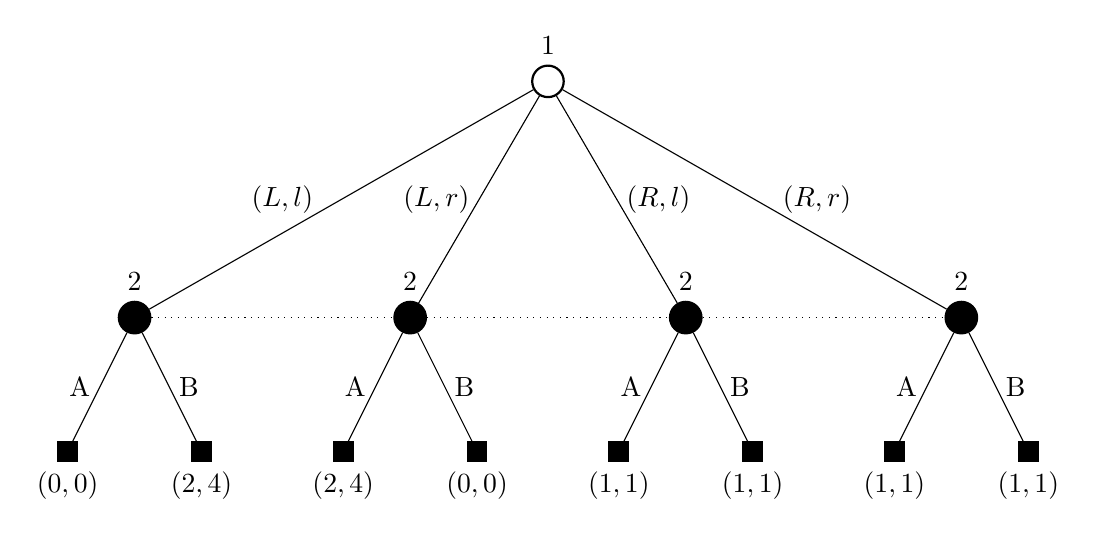
\begin{tikzpicture}[
chance/.style={circle, draw=black, fill=black, thick, minimum size = 6mm},
player1/.style={circle, draw=black, thick, minimum size = 4mm},
player2/.style={circle, draw=black, fill=black, thick, minimum size=4mm},
terminal/.style={rectangle, draw=black, fill=black, thick, minimum size=2mm},
level 1/.style={sibling distance=35mm, level distance=30mm},
level 2/.style={sibling distance=17mm, level distance=17mm},
]
\node[player1] [label=$1$] {}
	child { node (A) [player2] [label=above:{$2$}]  {}
    	child { node [terminal] [label=below:{$(0,0)$}] {}
        		edge from parent node[left] {A} }
        child { node [terminal] [label=below:{$(2,4)$}] {}
        		edge from parent node[right] {B} }
        edge from parent node[left] {$(L, l)\ \ $}
    }
    child { node (B) [player2] [label=above:{$2$}] {}
    	child { node [terminal] [label=below:{$(2,4)$}] {}
        		edge from parent node[left] {A} }
        child { node [terminal] [label=below:{$(0,0)$}] {}
        		edge from parent node[right] {B} }
        edge from parent node[left] {$(L, r)$}
    }
    child { node (C) [player2] [label=above:{$2$}] {}
    	child { node [terminal] [label=below:{$(1,1)$}] {}
        		edge from parent node[left] {A} }
        child { node [terminal] [label=below:{$(1,1)$}] {}
        		edge from parent node[right] {B} }
        edge from parent node[right] {$(R, l)$}
    }
    child { node (D) [player2] [label=above:{$2$}] {}
    	child { node [terminal] [label=below:{$(1,1)$}] {}
        		edge from parent node[left] {A} }
        child { node [terminal] [label=below:{$(1,1)$}] {}
        		edge from parent node[right] {B} }
        edge from parent node[right] {$\ \ (R, r)$}
    };
\draw[dotted] (A) -- (B) -- (C) -- (D);
\end{tikzpicture}
\caption{Árbol correspondiente a la forma normal de la Tabla \ref{table:fextensiva-a-fnormal}.}
\label{fig:arbol-de-tabla}
\end{center}
\end{figure}

\section{Estrategias de Comportamiento}

En juegos en forma extensiva, el jugador puede utilizar un tipo de estrategia diferente a la presentada anteriormente, y la cual es denominada estrategia de comportamiento (Definición \ref{def:estrategia-comportamiento}). Una estrategia de comportamiento para el jugador $i$ especifica una distribución de probabilidad sobre las acciones disponibles en cada conjunto de información del jugador $i$. Esto difiere a las estrategias mixtas que representan una distribución de probabilidad sobre las estrategias puras de un jugador \cite[p. 212]{bib:course-game-theory}. 

\begin{definition}
\label{def:estrategia-comportamiento}
Una \textbf{estrategia de comportamiento} para el jugador $i$ consiste en una distribución de probabilidad para cada conjunto de información $I_i \in \mathcal{I}_i$ sobre el conjunto $A(I_i)$ que pueden ejecutarse en $I_i$.
Es decir, una estrategia de comportamiento es una tupla $(\sigma^b_i(I_i))_{I_i \in \mathcal{I}_i}$ donde $\sigma^b_i(I_i) \in \Delta(A(I_i))$.
\end{definition}

Sea $B^i = \prod_{I_i \in \mathcal{I}_i} \Delta(A(I_i))$ el conjunto de todas las posibles estrategias de comportamiento del jugador $i$. Si $\sigma_i^b \in B^i$, $\sigma_i^b(I_i) \in \Delta(A(I_i))$ es una distribución de probabilidad sobre $A(I_i)$ mientras que $\sigma_i^b(I_i)(a)$ es la probabilidad de elegir la acción $a$ dada una historia $h \in I_i$.

\begin{definition}
Un \textbf{perfil estratégico de comportamiento} $\sigma^b$ es una estrategia de comportamiento para cada jugador.
\end{definition}

El conjunto de todos los perfiles estratégicos de comportamiento es $B = \prod_{i \in N} B^i$. Si $\sigma^b \in B$, la utilidad esperada de la estrategia $\sigma^b$ para el jugador $i$ es
\[ u_i(\sigma^b)\ =\ \sum_{s \in S} \sigma_b(s)u_i(s) \]
donde $\sigma_i^b(s_i) = \prod_{I_i \in \mathcal{I}_i} \sigma_i^b(I_i)(s_i(I_i))$, y $\sigma^b(s) =  \prod_{i \in N} \sigma_i^b(s_i)$.

Con las definiciones proporcionadas se puede definir los conceptos de equilibrio de Nash y aproximación de equilibrio de Nash para juegos en forma extensiva.

\begin{definition}
Sea $\Sigma=\prod_{i\in N}\Sigma_i$ el conjunto de perfiles mixtos o de comportamiento, según sea el caso, para los jugadores en $N$.
Para $\varepsilon\geq 0$, se dice que un perfil estratégico $\sigma \in \Sigma$ es un \textbf{$\varepsilon$-equilibrio de Nash} si y sólo si para todo jugador $i$ y perfil $\sigma'_i\in\Sigma_i$,
\begin{alignat}{1}
u_i(\sigma) + \varepsilon\ \geq\ u_i(\sigma'_i, \sigma_{-i}) \,.
\end{alignat}
El perfil $\sigma\in\Sigma$ es un \textbf{equilibrio de Nash} si y sólo si $\sigma$ es un $0$-equilibrio de Nash.
\end{definition}

En el Ejemplo~\ref{ex:informacion-incompleta} se tienen $4$ estrategias puras para el jugador $1$ (Tabla \ref{table:estrategias-puras}). Una estrategia mixta $\sigma^m_1$ es una distribución de probabilidad sobre el conjunto $\{s_1, s_2, s_3, s_4\}$, donde las probabilidades son $\sigma^m_1(s_1)$, $\sigma^m_1(s_2)$, $\sigma^m_1(s_3)$ y $\sigma^m_1(s_4)$. Por otra parte una estrategia de comportamiento $\sigma^b_1$ son dos distribuciones de probabilidad, $\sigma^b_1(I^1)$ y $\sigma^b_1(I_2)$, sobre los conjuntos $A(I^1) = \{L, R\}$ y $A(I^2) = \{l, r\}$ respectivamente.


\subsection*{Equilibrio de Nash en el Juego de Kuhn Poker}

En el juego de Kuhn Poker si ambos jugadores juegan de forma óptima, es decir, acorde a un equilibrio de Nash, entonces el jugador $2$ tiene una ganancia esperada de $\frac{1}{18}$ por mano, como se prueba en \cite{bib:kuhn-poker}. El conjunto de equilibrios de Nash se resume en la Tabla~\ref{tab:estrategia-kuhn-poker}, donde los conjuntos de información fueron enumerados en un orden de búsqueda por profundidad (DFS).

\begin{table}[h]
\begin{center}
    \caption{Equilibrio de Nash para el juego de Kuhn Poker. Cada fila de la tabla corresponde con uno o varios conjuntos de información que se denotan con enteros (enumerados utilizando un procedimiento de búsqueda en profundidad sobre el árbol del juego). El equilibro de Nash corresponde con una distribución aleatoria sobre las acciones pasar y apostar la cuál depende de un parámetro $\alpha \in \left[ 0,\frac{1}{3} \right]$.}
    \label{tab:estrategia-kuhn-poker}
    \begin{tabular}{c r r}
        \toprule
        \multirow{2}{*}{Conjunto de} & \multicolumn{2}{c}{Equilibrio de Nash}  \\ \cmidrule(l){2-3}
        información & pasar & apostar \\ 
        \midrule
         $1$ & $1-\alpha$ & $\alpha$ \\
         $2, 3, 6, 10$ & $1$ & $0$ \\
         $4$ & $\frac{2}{3}$ & $\frac{1}{3}$ \\
         $5, 7, 12$ & $0$ & $1$ \\
         $8$ & $\frac{2}{3}$ & $\frac{1}{3}$ \\
         $9$ & $\frac{2}{3} - \alpha$ & $\alpha + \frac{1}{3}$ \\
        $11$ & $1 - 3 \alpha$ & $3 \alpha$ \\ \bottomrule
    \end{tabular}
\end{center}
\end{table}

El primer jugador tiene infinitas estrategias óptimas, las cuales pueden ser representadas por la elección de un parámetro $\alpha \in \left[ 0, \frac{1}{3} \right]$. Una vez elegido este parámetro, el primer jugador en su primera jugada debe apostar con probabilidad $\alpha$ cuando su carta tenga el número $1$, apostar con una probabilidad $3 \alpha$ cuando tenga el número $3$ y pasar siempre cuando tenga el número $2$. Si el primer jugador tiene un segundo turno, debe pasar siempre que tenga el número $1$, apostar cuando tiene el número $3$, y en el caso que tenga el número $2$ debe apostar con probabilidad $\alpha + \frac{1}{3}$.

El segundo jugador tiene una única estrategia mixta óptima: apostar siempre que tenga el número $3$. Cuando tenga el número $1$, pasar siempre que el primer jugador haya apostado y apostar con probabilidad $\frac{1}{3}$ en caso contrario. Cuando tenga el número $2$, debe pasar cuando el oponente haya pasado previamente y apostar con probabilidad $\frac{2}{3}$ en caso contrario. La figura \ref{fig:kuhn-poker-estrategias} muestra el árbol con las distribuciones de probabilidad de las estrategias previamente descritas en cada uno de los nodos alcanzables en el juego.

\begin{figure}[h]
\begin{center}
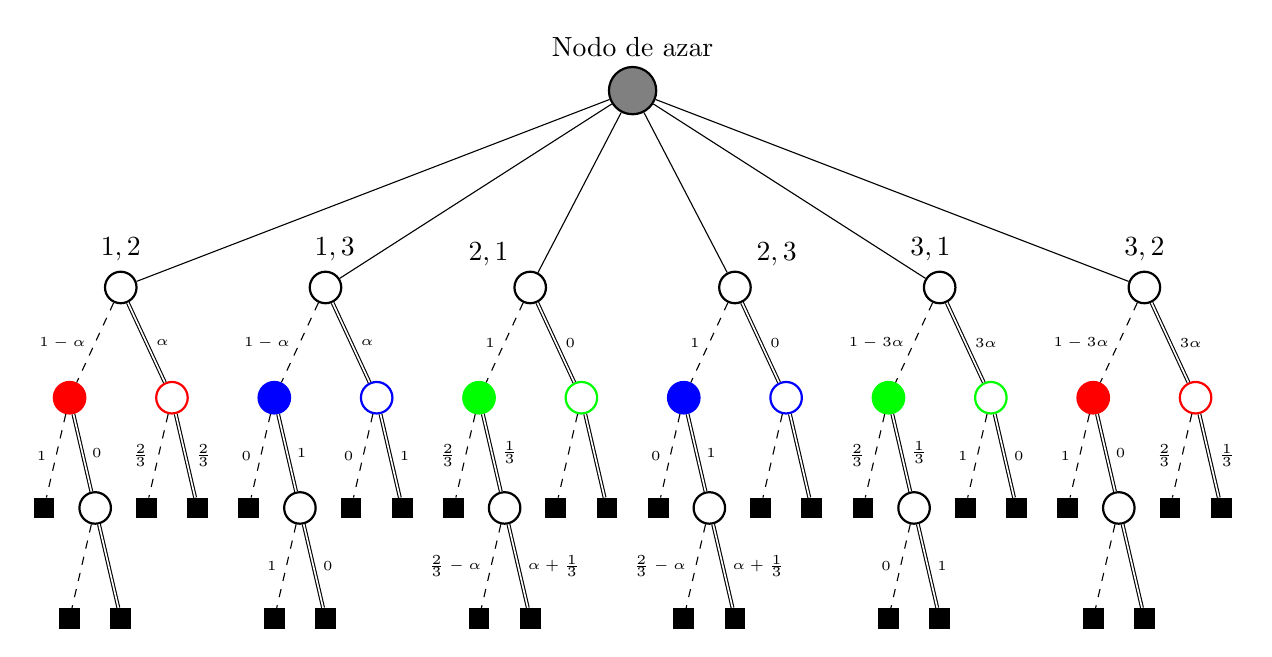
\begin{tikzpicture}[
chance/.style={circle, draw=black, fill=gray, thick, minimum size = 6mm},
player1/.style={circle, draw=black, solid, thick, minimum size = 4mm},
player2/.style={circle, thick, minimum size=4mm},
terminal/.style={rectangle, draw=black, solid, fill=black, thick, minimum size=2mm},
level 1/.style={sibling distance=26mm, level distance=25mm},
level 2/.style={sibling distance=13mm, level distance=14mm},
level 3/.style={sibling distance=6.5mm, level distance=14mm},
]
\node[chance] [label=above:{Nodo de azar}] {} {
	child {node [player1] (P1) [label=above:{$1, 2$}]{}
		child { node [player2] [draw=red, fill=red] {} 
				child { node [terminal] {}
						edge from parent [dashed] node [left, draw=none] {\tiny{$1$}} {} }
				child { node [player1] (A) {} 
						child { node [terminal] {}
								edge from parent [dashed] {} }
						child { node [terminal] {} 
								edge from parent [solid, double] {} }
						edge from parent [solid, double] node [right, draw=none] {\tiny{$0$}}  {}
				}
				edge from parent [dashed] node [left, draw=none] {\tiny{$1-\alpha$}}  {}
		}
		child { node [player2] [draw=red] {} 
				child { node [terminal]  {}
						edge from parent [dashed] node [left, draw=none] {\tiny{$\frac{2}{3}$}} {} }
				child { node [terminal]  {}
						edge from parent [solid, double] node [right, draw=none] {\tiny{$\frac{2}{3}$}} {} }
				edge from parent [solid, double] node [right, draw=none] {\tiny{$\alpha$}}{}
		}
	}
	child {node [player1] (P2) [label=above:{$\ \ 1, 3$}]{}
		child { node [player2] [draw=blue, fill=blue] {} 
				child { node [terminal] {}
						edge from parent [dashed] node [left, draw=none] {\tiny{$0$}} {} }
				child { node [player1] (B) {} 
						child { node [terminal] {}
								edge from parent [dashed] node [left, draw=none] {\tiny{$1$}} {} }
						child { node [terminal] {}
								edge from parent [solid, double] node [right, draw=none] {\tiny{$0$}} {} }
						edge from parent [solid, double] node [right, draw=none] {\tiny{$1$}} {}
				}
				edge from parent [dashed] node [left, draw=none] {\tiny{$1-\alpha$}} {}
		}
		child { node [player2] [draw=blue] {} 
				child { node [terminal] {}
						edge from parent [dashed] node [left, draw=none] {\tiny{$0$}} {} }
				child { node [terminal] {}
						edge from parent [solid, double] node [right, draw=none] {\tiny{$1$}} {} }
				edge from parent [solid, double] node [right, draw=none] {\tiny{$\alpha$}} {}
		}
	}
	child {node [player1] (P3) [label=135:{$2, 1$}]{}
		child { node [player2] [draw=green, fill=green] {} 
				child { node [terminal] {}
						edge from parent [dashed] node [left, draw=none] {\tiny{$\frac{2}{3}$}} {} }
				child { node [player1] (C) {} 
						child { node [terminal] {}
								edge from parent [dashed] node [left, draw=none] {\tiny{$\frac{2}{3}-\alpha$}} {} }
						child { node [terminal] {} 
                        		edge from parent [solid, double] node [right, draw=none] {\tiny{$\alpha+\frac{1}{3}$}} {} }
						edge from parent [solid, double] node [right, draw=none] {\tiny{$\frac{1}{3}$}} {}
				}
				edge from parent [dashed] node [left, draw=none] {\tiny{$1$}} {}
		}
		child { node [player2] [draw=green] {} 
				child { node [terminal] {}
						edge from parent [dashed] {} }
				child { node [terminal] {}
						edge from parent [solid, double] {} }
				edge from parent [solid, double] node [right, draw=none] {\tiny{$0$}} {}
		}
	}
	child {node [player1] (P4) [label=45:{$2, 3$}]{}
		child { node [player2] [draw=blue, fill=blue]{} 
				child { node [terminal] {}
						edge from parent [dashed] node [left, draw=none] {\tiny{$0$}} {} }
				child { node [player1] (D) {} 
						child { node [terminal] {}
								edge from parent [dashed] node [left, draw=none] {\tiny{$\frac{2}{3}-\alpha$}} {} {} }
						child { node [terminal] {}
								edge from parent [solid, double] {} node [right, draw=none] {\tiny{$\alpha+\frac{1}{3}$}} {} }
						edge from parent [solid, double] node [right, draw=none] {\tiny{$1$}} {}
				}
				edge from parent [dashed] node [left, draw=none] {\tiny{$1$}} {}
		}
		child { node [player2] [draw=blue] {} 
				child { node [terminal] {}
						edge from parent [dashed] {} }
				child { node [terminal] {}
						edge from parent [solid, double] {} }
				edge from parent [solid, double] node [right, draw=none] {\tiny{$0$}} {}
		}
	}
	child {node [player1] (P5) [label=above:{$3, 1\ \ $}]{}
		child { node [player2] [draw=green, fill=green] {} 
				child { node [terminal] {}
						edge from parent [dashed] node [left, draw=none] {\tiny{$\frac{2}{3}$}} {} }
				child { node [player1] (E) {} 
						child { node [terminal] {}
								edge from parent [dashed] node [left, draw=none] {\tiny{$0$}} {} }
						child { node [terminal] {}
								edge from parent [solid, double] node [right,draw=none] {\tiny{$1$}} {} }
						edge from parent [solid, double] node [right, draw=none] {\tiny{$\frac{1}{3}$}} {}
				}
				edge from parent [dashed] node [left, draw=none] {\tiny{$1-3 \alpha$}} {}
		}
		child { node [player2] [draw=green] {} 
				child { node [terminal] {}
						edge from parent [dashed] node [left, draw=none] {\tiny{$1$}} {} }
				child { node [terminal] {}
						edge from parent [solid, double] node [right, draw=none] {\tiny{$0$}} {} }
				edge from parent [solid, double] node [right, draw=none] {\tiny{$3 \alpha$}} {}
		}
	}
	child {node [player1] (P6) [label=above:{$3, 2$}]{}
		child { node [player2]  [draw=red, fill=red] {} 
				child { node [terminal] {}
						edge from parent [dashed] node [left, draw=none] {\tiny{$1$}} {} }
				child { node [player1] (F) {} 
						child { node [terminal] {}
								edge from parent [dashed] {}}
						child { node [terminal]  {}
								edge from parent [solid, double] {} }
						edge from parent [solid, double] node [right, draw=none] {\tiny{$0$}} {}
				}
				edge from parent [dashed] node [left, draw=none] {\tiny{$1-3\alpha$}} {}
		}
		child { node [player2]  [draw=red] {} 
				child { node [terminal]  {}
						edge from parent [dashed] node [left, draw=none] {\tiny{$\frac{2}{3}$}} {} }
				child { node [terminal] {}
						edge from parent [solid, double] node [right, draw=none] {\tiny{$\frac{1}{3}$}} {} }
				edge from parent [solid, double] node [right, draw=none] {\tiny{$3\alpha$}} {}
		}
	}
};
\end{tikzpicture}
\caption{Equilibrios de Nash para el juego de Kuhn Poker. Las etiquetas sobre las aristas del árbol indican la probabilidad de escoger dicha acción en cada nodo para un parámetro $\alpha \in \left[ 0,\frac{1}{3} \right]$.}
\label{fig:kuhn-poker-estrategias}
\end{center}
\end{figure}


\section{Probabilidad de Alcanzar una Historia y un Conjunto de Información}
\label{sec:probabilidad-historia}

Sea $\sigma$ un perfil estratégico mixto o de comportamiento el cual agrega una estrategia $\sigma_i$ para cada jugador $i$. Definimos la probabilidad de alcanzar la historia $h$ cuando los jugadores utilizan $\sigma$ como la multiplicación de la probabilidad de que cada acción $a$ en la historia $h$ ocurra, cuando dicha acción es seleccionada por un jugador $i$ o por el azar, según sea el caso. Formalmente, en símbolos, dicha probabilidad se expresa de la siguiente forma:
\begin{alignat}{1}
  \pi^\sigma(h)\
    =\ \prod_{i\in N} \left\{ \prod_{(h',a)\sqsubseteq h : P(h')=i} \sigma_i(h')(a) \right\}\ \times \prod_{(h',a)\sqsubseteq h : P(h')=c} f_c(a|h') \,. 
\end{alignat}
En esta expresión la historia $h$ es descompuesta en prefijos $(h',a)$ los cuales definen los términos en el producto; término para $(h',a)$ es $\sigma_i(h')(a)$ cuando le toca jugar a $i$ (i.e., $P(h')=i$) o $f_c(a|h')$ cuando le toca jugar al azar (i.e., $P(h')=c$).

La probabilidad $\pi^\sigma(h)$ la podemos expresar como un producto de probabilidades para cada jugador $i\in N$ y una probabilidad $\pi^c(h)$ que corresponde al azar la cual no depende de $\sigma$:
\begin{alignat}{1}
  \pi^\sigma(h)\ =\ \left\{\prod_{i\in N} \pi^\sigma_i(h)\right\} \times \pi^c(h)
\end{alignat}
donde $\pi^\sigma_i(h) = \prod_{(h',a)\sqsubseteq h : P(h')=i} \sigma_i(h')(a)$ y $\pi^c(h)=\prod_{(h',a)\sqsubseteq h : P(h')=c} f_c(a|h')$. Estas probabilidades les podemos dar interpretación: $\pi^\sigma_i(h)$ es la probabilidad de alcanzar la historia $h$ cuando el jugador $i$ utilizar la estrategia $\sigma_i$ y los otros jugadores, incluyendo el azar, juegan para alcanzar $h$, y $\pi^c(h)$ es la probabilidad de alcanzar la historia $h$ cuando todos los jugadores juegan para alcanzar $h$. Similarmente, definimos $\pi^\sigma_{-i}(h)=\pi^\sigma(h) / \pi^\sigma_i(h)$ que puede interpretarse como la probabilidad de alcanzar $h$ cuando todos los jugadores excepto $i$ utilizan $\sigma_{-i}$, y el jugador $i$ juega para alcanzar la historia $h$.

Las probabilidades arriba definidas pueden agregarse para definir probabilidades de alcanzar conjuntos de información, ya que un conjunto de información no es otra cosa que un subconjunto de historias. Así, definimos, 
$\pi^\sigma(I)=\sum_{h\in I}\pi^\sigma(h)$, $\pi^\sigma_i(I)=\sum_{h\in I}\pi^\sigma_i(h)$, y $\pi^\sigma_{-i}(I)=\sum_{h\in I}\pi^\sigma_{-i}(h)$.


Finalmente, para un perfil estratégico $\sigma$, definimos la ganancia esperada del jugador $i$ cuando todos los jugadores utilizan $\sigma$ como $u_i(\sigma) = \sum_{z \in Z} u_i(z)\pi^\sigma(z)$. 

\section{Perfect Recall}

El concepto de \textit{perfect recall} hace referencia a juegos en los cuales, en cualquier punto todo jugador \textit{recuerda} lo que sabía previamente \cite[p.~203]{bib:course-game-theory}. En particular, cada jugador recuerda los movimientos públicos que se han hecho durante el juego. La definición de \textit{perfect recall} puede ser dada mediante el árbol del juego \cite{bib:conceptos-basicos} o mediante la subsecuencia correspondiente a los nodos de un jugador \cite[p.~203]{bib:course-game-theory} y \cite[p.~44]{bib:handbook-blai}. Sin embargo, se utiliza una definición equivalente, proporcionada en la Definición \ref{def:perfect-recall}.

\begin{definition}
\label{def:perfect-recall}
Se dice que el jugador $i$ tiene \textbf{\textit{perfect recall}} en el juego $\Gamma$ (en forma extensiva) si para cualquier par de historias $h_1, h_2$ con $P(h_1) = P(h_2) = i$, tales que $I(h_1) = I(h_2)$ las siguientes condiciones se cumplen:
\begin{alignat}{1}
& h \sqsubseteq h_1\ \implies\ (\exists h' \sqsubseteq h_2 : I(h) = I(h')) \,,
\label{eq:condicion-1}\\
& (h_1, a) \sqsubseteq h\  \land\ (h_2, b)\sqsubseteq h'\ \land\ a \neq b\ \  \implies\ I(h) \neq I(h') \,.
\label{eq:condicion-2}
\end{alignat}
\end{definition}

Intuitivamente, las condiciones presentadas representan las siguientes propiedades del jugador $i$:
\begin{enumerate}[noitemsep]
\item \textit{El jugador $i$ recuerda lo que sabía} (Ecuación \ref{eq:condicion-1}): en cualquier momento el jugador $i$ recuerda si pasó o no por un conjunto de información específico. En efecto, si dos secuencias, por ejemplo $h_1$ y $h_2$, pertenecen al mismo conjunto de información y para llegar a $h_1$ se debe pasar por $h$, entonces, para llegar a $h_2$, se debe pasar por algún $h'$ tal que $h'$ y $h$ pertenezcan al mismo conjunto de información. 

\item \textit{El jugador $i$ recuerda lo que eligió} (Ecuación \ref{eq:condicion-2}): si desde una historia $h$ el jugador elige $a$, entonces el jugados estaría  en un conjunto de información diferente si en ese punto hubiese elegido la acción $b \neq a$.
\end{enumerate}

Los juegos presentados previamente: Ejemplo \ref{ex:game-allocation}, Ejemplo \ref{ex:informacion-incompleta} y Kuhn Poker son todos juegos con \textit{perfect recall}. El Ejemplo \ref{ex:imperfect-recall} muestra un juego con \textit{imperfect recall}.

\begin{example} (\cite{bib:conceptos-basicos})
\label{ex:imperfect-recall}
Considere un juego de dos jugadores de suma cero en el cual el jugador $1$ consta de $2$ personas: Alicia y su esposo Bernardo, y el jugador $2$ consta de una sóla persona: Zoe. Se tienen dos cartas con los números $1$ y $2$ que son repartidas aleatoriamente entre Alicia y Zoe. La persona con la carta más alta recibe \$1 de la persona con la carta más baja, y ésta decide si sigue jugando (C) o para el juego (P). Si el juego continúa, Bernardo, sin saber el resultado de la repartición inicial de las cartas, decide si Alicia y Zoe intercambian (I) sus cartas o mantienen las mismas cartas (M). Nuevamente, quien posea la carta más alta recibe \$1 de quien posea la carta más baja, y el juego termina.
\end{example}

 La Figura \ref{fig:imperfect-recall} representa el juego en forma extensiva. Note que cuando es el turno de Bernardo, él no sabe quien tiene la carta más alta, cosa que su esposa sí sabía en el turno anterior. Al considerar a la pareja como un sólo jugador, se obtiene que el jugador $1$ \textit{olvidó} como fueron repartidas las cartas. En efecto, el jugador $1$ tiene dos conjuntos de información $I^1_1 = \{(2-1) \}$ e $I^2_1 = \{(2-1,\ C),\ (1-2,\ C) \}$. En particular, no se cumple la primera condición (Ecuación \ref{eq:condicion-1}), pues la secuencia $(2-1) \sqsubset (2-1,\ C)$, pero no existe una subsecuencia de $(1-2,\ C)$ que pertenezca a $I^1_1$.

\begin{figure}[h]
\begin{center}
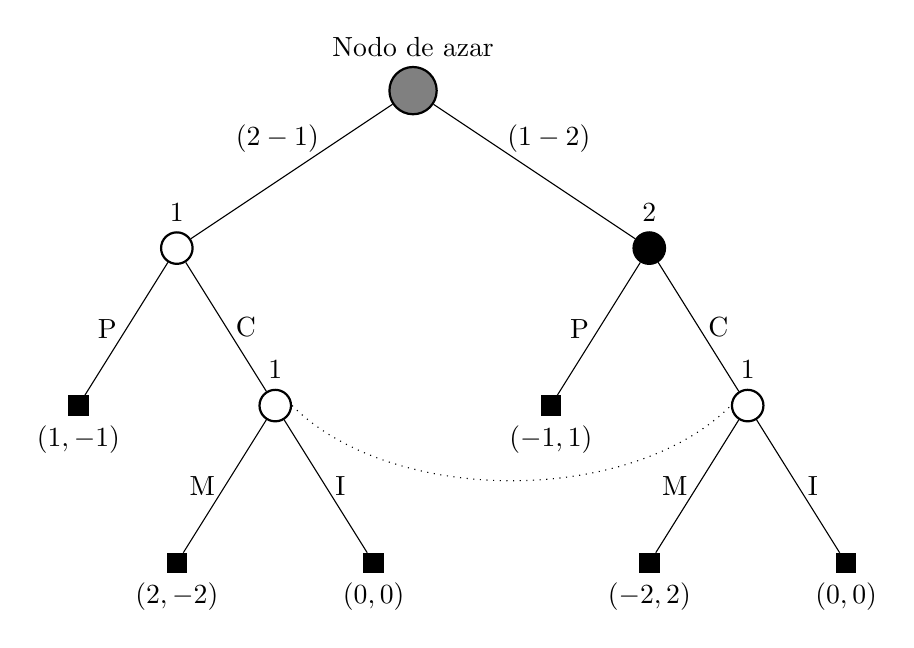
\begin{tikzpicture}[
chance/.style={circle, draw=black, fill=gray, thick, minimum size = 6mm},
player1/.style={circle, draw=black, thick, minimum size = 4mm},
player2/.style={circle, draw=black, fill=black, thick, minimum size=4mm},
terminal/.style={rectangle, draw=black, fill=black, thick, minimum size=2mm},
level 1/.style={sibling distance=60mm, level distance=20mm},
level 2/.style={sibling distance=25mm, level distance=20mm},
level 3/.style={sibling distance=25mm, level distance=20mm},
]

\node[chance] [label = {Nodo de azar}] {}
	child { node[player1] [label=above:{$1$}] {}
    	child { node[terminal] [label=below:{$(1, -1)$}] {} 
        		edge from parent node[left] {P} }
        child { node (A) [player1] [label=above:{$1$}] {}
        		child { node[terminal] [label=below:{$(2, -2)$}] {}
                		edge from parent node[left] {M} }
                child { node[terminal] [label=below:{$(0,  0)$}] {}
                		edge from parent node[right] {I} }
        		edge from parent node[right] {C}
              }
    	edge from parent node[left] [label=above:{$(2-1)\ $}] {}
    }
    child{ node[player2] [label=above:{$2$}] {}
    	child { node (C) [terminal] [label=below:{$(-1, 1)$}] {} 
        		edge from parent node[left] {P} }
        child { node (B) [player1] [label=above:{$1$}] {}
        		child { node[terminal] [label=below:{$(-2, 2)$}] {}
                		edge from parent node[left] {M} }
                child { node[terminal] [label=below:{$(0,  0)$}] {}
                		edge from parent node[right] {I} }
        		edge from parent node[right] {C}
              }
    	edge from parent node[right] [label=above:{$\ (1-2)$}] {}
    };

\draw[dotted] (A.east) .. controls ++(135:-18mm) and ++(45:-18mm) .. (B.west);
\end{tikzpicture}
\caption{Árbol de la forma extensiva del juego con \textit{imperfect recall} presentado en el Ejemplo \ref{ex:imperfect-recall}. P representa la acción de parar el juego y C de continuarlo. M representa la acción de mantener las cartas obtenidas inicialmente e I representan la acción de intercambiarlas.}
\label{fig:imperfect-recall}
\end{center}
\end{figure}
Una pregunta de interés es si es posible sustituir una estrategia mixta por una estrategia de comportamiento o viceversa. Para esto, es necesario establecer una definición de equivalencia entre estrategias, y la alcanzabilidad de una historia bajo una estrategia pura.

\begin{definition}
\label{def:equivalencia-estrategias}
Se dice que dos estrategias $\sigma$ y $\sigma'$ son equivalentes si la probabilidad de alcanzar cualquier historia terminal es la misma; i.e., $\pi^\sigma(z) = \pi^{\sigma'}(z)$ para todo $z \in Z$.
\end{definition}

\begin{definition}
\label{def:alcanzabilidad-historia}
Sea $s_i \in S_i$ una estrategia pura del jugador $i$ e $I_i \in \mathcal{I}$ un conjunto de información de dicho jugador. Se dice que $I_i$ es alcanzable bajo $s_i$ si existe una historia $h \in H$ tal que $h \in I_i$ y para toda historia (prefijo) $h' \sqsubset h$ se cumple que: si $P(h') = i$, entonces $(h', s_i(I(h')))$ $\sqsubset$ $h$ y si $P(h') = c$ entonces existe una acción $a$ tal que $(h', a) \sqsubset h$ y la probabilidad de elegir la acción $a$ en $h'$ es positiva, i.e., $f_c(a|h') > 0$. 
\end{definition}

La definición anterior puede ser aplicada tanto a perfiles estratégicos como a estrategias para un jugador en particular, utilizando la definición de $\pi^\sigma(z)$ correspondiente. Las preguntas que se desean responder son las siguientes: (i) ?`Dada una estrategia mixta $\sigma^m$, existe una estrategia de comportamiento $\sigma^b$ tal que $\sigma^m$ y $\sigma^b$ son equivalentes? (ii) ?`Dada una estrategia de comportamiento $\sigma^b$, existe una estrategia mixta $\sigma^m$ tal que $\sigma^b$ y $\sigma^m$ son equivalentes?. Los Teoremas \ref{theo:comportamiento-a-mixta} y \ref{theo:mixta-a-comportamiento} responden estas interrogantes.

El Teorema \ref{theo:comportamiento-a-mixta} establece que si para cualquier camino de la raíz a un nodo no se pasa $2$ o más veces el mismo conjunto de información, entonces para cualquier estrategia de comportamiento existe una estrategia mixta equivalente. Por otra parte, el Teorema \ref{theo:mixta-a-comportamiento} establece que si todos los jugadores tienen \textit{perfect recall} entonces para toda estrategia mixta existe una estrategia de comportamiento equivalente. En particular, si se tiene \textit{perfect recall} entonces ningún camino pasa por el mismo conjunto de información más de una vez y, por lo tanto, para cualquier estrategia de comportamiento también existe una estrategia de comportamiento equivalente. En efecto, las estrategias de comportamiento es una forma compacta de representar las estrategias mixtas en este tipo de juegos.

\begin{theorem}
\label{theo:comportamiento-a-mixta}
Si para el jugador $i$ se cumple que $I(h')\neq I(h)$ para cualquier
par de historias $h$ y $h'$ tal que $h'\sqsubset h$ y $P(h)=P(h')=i$, entonces para cualquier estrategia de comportamiento $\sigma^b_i \in B^i$ para el jugador $i$, existe una estrategia mixta $\sigma^m_i$ que es \textbf{equivalente} a $\sigma^b_i$. En particular, la estrategia mixta $\sigma^m_i$ viene dada por:
\begin{alignat}{1}
\sigma^m_i(s_i)\ :=\ \prod_{I_i \in \mathcal{I}_i} \sigma^b_i(I_i)(s_i(I_i)) \,. \label{eq:comportamiento-a-mixta}
\end{alignat}
\end{theorem}

El Ejemplo~\ref{ex:imperfect-recall-2} muestra un juego en el que no se cumple la condición del Teorema \ref{theo:comportamiento-a-mixta}, es decir, un juego en el que una historia pasa más de una vez sobre mismo conjunto de información. En este tipo de juegos se obtiene que el poder expresivo de las estrategia mixtas y las estrategias de comportamiento no son comparables.

\begin{example}[{\cite[p.~44]{bib:handbook-blai}}]
\label{ex:imperfect-recall-2}
Considere un juego en forma extensiva de dos jugadores definido por:
\begin{alignat}{1}
    &H = \{ \emptyset, (L), (R), (L,L), (L,R), (R, U), (R, D)\} \,, \\
    &P(\emptyset) = P(L) = 1, \ P(R) = 2 \,, \\
    &f(L, L) = (1, 0), \ f(L, R) = (100, 100), \ f(R, U) = (5, 1), \ f(R, D) = (2, 2) \,, \\
    &\mathcal{I}_1 = \{ \{ \emptyset, (L)\} \}, \ \mathcal{I}_2 = \{ \{ R \} \} \,.
\end{alignat}
El árbol de este juego, con \textit{imperfect recall}, se muestra en la Figura \ref{fig:imperfect-recall-2}.
\end{example}

\begin{figure}[h]
\begin{center}
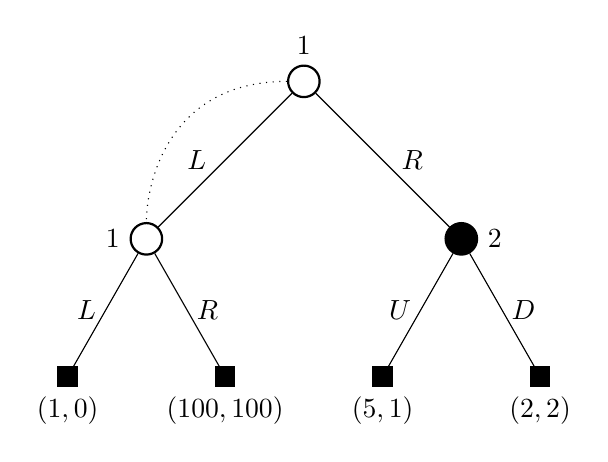
\begin{tikzpicture}[
chance/.style={circle, draw=black, fill=black, thick, minimum size = 6mm},
player1/.style={circle, draw=black, thick, minimum size = 4mm},
player2/.style={circle, draw=black, fill=black, thick, minimum size=4mm},
terminal/.style={rectangle, draw=black, fill=black, thick, minimum size=2mm},
level 1/.style={sibling distance=40mm, level distance=20mm},
level 2/.style={sibling distance=20mm, level distance=17.5mm},
]
\node[player1] (A) [label=$1$] {}
	child { node (B) [player1] [label=left:{$1$}]  {}
    	child { node [terminal] [label=below:{$(1,0)$}] {}
        		edge from parent node[left] {$L$} }
        child { node [terminal] [label=below:{$(100,100)$}] {}
        		edge from parent node[right] {$R$} }
        edge from parent node[left] {$L\ $}
    }
    child { node [player2] [label=right:{$2$}] {}
    	child { node [terminal] [label=below:{$(5,1)$}] {}
        		edge from parent node[left] {$U$} }
        child { node [terminal] [label=below:{$(2,2)$}] {}
        		edge from parent node[right] {$D$} }
        edge from parent node[right] {$\ R$}
    };
\draw [dotted]
(A.west) .. controls ++(left:+15mm) and ++(90:+5mm) .. (B.north);
\end{tikzpicture}
\caption{Árbol de la forma extensiva del juego con \textit{imperfect recall} presentado en el Ejemplo~\ref{ex:imperfect-recall-2}. Observe que existe una historia que pasa dos veces sobre el mismo conjunto de información.}
\label{fig:imperfect-recall-2}
\end{center}
\end{figure}

Note que la historia $(L, L)$ atraviesa $2$ veces el único conjunto de información del jugador $1$. La situacion se corresponde con que el jugador 1 \textit{olvida} la elección entre $L$ o $R$ que hizo previamente cuan elige $L$ en la raíz. En este juego el jugador $1$ tiene $2$ posibles estrategias puras, elegir $L$ o $R$. Por lo tanto, en una estrategia mixta él elige una de estas $2$ acciones según alguna distribución de probabilidad. Sin embargo, luego de la elección siempre realizará la misma jugada cuando tenga que tomar una decisión. En particular, la historia $(L,R)$ no puede ocurrir y el pago de ($100$, $100$) es irrelevante en el contexto de estrategias mixtas.

En este juego en particular, se tiene que la estrategia $R$ es mejor para el jugador $1$, independientemente de la elección del jugador $2$, y la estrategia pura $D$ del jugador $2$ es mejor respuesta ante cualquier estrategia de $1$. Luego, el único equilibrio de Nash (de estrategias mixtas) es $\sigma = (\sigma_1, \sigma_2)$, donde $\sigma_1(L) = 0$, $\sigma_1(R) = 1$, $\sigma_2(D) = 1$ y $\sigma_2(U) = 0$, cuya ganancia es igual a $2$ para ambos jugadores.

Por otra parte, si se consideran estrategias de comportamiento, se debe elegir una distribución $(p, 1-p)$ para elegir $L$ y $R$. En este caso la historia $(L, R)$ tiene una probabilidad de $p(1-p)$ de ser elegida y su pago juega un papel relevante al momento de elegir la estrategia óptima. La estrategia mencionada previamente ya no es un equilibrio de Nash con respecto al conjunto de estrategias de comportamientos. De hecho, el equilibrio se obtiene cuando $p = \frac{98}{198}$ y el jugador $2$ siempre elige $D$.
Note que para esta estrategia de comportamiento, no existe una estrategia mixta equivalente; sin embargo, en juegos que cumplen la condición del Teorema \ref{theo:comportamiento-a-mixta} para el jugador $i$, toda estrategia de comportamiento para $i$ tienen una estrategia mixta para $i$ que es equivalente.

%\medskip

Se considerará nuevamente el Ejemplo \ref{ex:imperfect-recall}, el cual no tiene \textit{perfect recall}. Las estrategias puras para el jugador $1$ son (P, I), (P, M), (C, I), (C, M), y las estrategias puras para el jugador $2$ son (P) y (C). Luego, la Tabla \ref{table:imperfect-recall} es la tabla correspondiente a la forma normal del juego, la cual incluye sólo la función de pago del jugador $1$, ya que al ser un juego de suma $0$, el pago del jugador $2$ está completamente determinado.

\begin{table}[h]
\begin{center}
\caption[Tabla de la forma normal para un juego con \textit{imperfect recall}]{Tabla de la forma normal para el Juego \ref{ex:imperfect-recall} con \textit{imperfect recall}.}
\label{table:imperfect-recall}
\begin{tabular}{l | r | r |}
\multicolumn{1}{c}{} & \multicolumn{1}{c}{(P)} & \multicolumn{1}{c}{(C)} \\ \cline{2-3}
(P, M)     & $0$ & $-0.5$ \\ \cline{2-3}
(P, I) & $0$ & $0.5$ \\ \cline{2-3}
(C, M)     & $0.5$ & $0$ \\ \cline{2-3}
(C, I) & $-0.5$ & $0$ \\ \cline{2-3}
\end{tabular}
\end{center}
\end{table}

Note que el pago que proporciona la estrategia (P, I) al jugador $1$ es siempre mayor o igual al pago que le proporciona la estrategia (P, M), sin importar lo que haga el jugador $2$. En este caso se dice que la estrategia (P, I) domina a la estrategia (P, M). Asimismo, para este jugador, la estrategia (C, M) domina a la estrategia (C, I). Por lo tanto, el jugador 1 se puede enfocar en encontrar una estragia mixta que no considere las estrategias (P, M) y (C, I). Supongamos que la estrategia del jugador 1 consiste en elegir las estrategias (P, I) y (C, M) con una probabilidad de $\frac{1}{2}$ cada una. La interrogante planteada es la siguiente ?`Existirá una estrategia de comportamiento equivalente a esta estrategia mixta?

La respuesta a la interrogante es no. Para observarlo, considere una estrategia de comportamiento en la que se elige parar el juego con probabilidad $\alpha$ y mantener las cartas con una probabilidad $\beta$. La probabilidad de elegir cada una de las estrategias puras del jugador 1 se observa en la Tabla~\ref{table:proba-ep}. En la estrategia mixta deseada la estrategia pura (P, M) tiene probabilidad $0$, por lo que $\alpha$ o $\beta$ debería ser $0$. Sin embargo, si $\alpha = 0$ la estrategia pura (P, I) tiene una probabilidad $0$ de ser elegida y si $\beta = 0$ entonces es imposible elegir la estrategia (C, M). Luego, no existe una estrategia de comportamiento equivalente a la estrategia mixta deseada. Sin embargo, esto no es un contraejemplo al Teorema~\ref{theo:mixta-a-comportamiento} ya que el juego no tiene \textit{perfect recall}.

\begin{table}[h]
\begin{center}
\caption[Probabilidades de las Estrategias Puras]{Probabilidades de cada estrategia pura dada una estrategia de comportamiento para el jugador $1$ del Ejemplo \ref{ex:imperfect-recall}.}
\label{table:proba-ep}
\begin{tabular}{c c c}
\toprule
& P ($\alpha$) & C ($1 - \alpha$) \\ \midrule
M ($\beta$)       & $\alpha\beta$     & $(1-\alpha)\beta$    \\
I ($1-\beta$) & $\alpha(1-\beta)$ & $(1-\alpha)(1-\beta)$\\ \bottomrule
\end{tabular}
\end{center}
\end{table}

\begin{theorem}
\label{theo:mixta-a-comportamiento}
Considere un juego finito de $N$ personas. Si el jugador $i$ tiene ``perfect recall",  entonces para cada estrategia mixta $\sigma^m_i \in \Delta(S_i)$ del jugador $i$, existe una estrategia de comportamiento $\sigma^b_i \in B^i$ equivalente a $\sigma^m_i$.
\end{theorem}


Se puede observar que cuando se tiene un juego con \textit{perfect recall}, se cumplen las condiciones de los Teoremas \ref{theo:mixta-a-comportamiento} y \ref{theo:comportamiento-a-mixta}. Por lo tanto se pueden intercambiar estrategias mixtas por estrategias de comportamiento y viceversa sin perder poder expresivo. Esto se enuncia con el Teorema \ref{theo:equivalencia-estrategias}.

\begin{theorem}[{ \cite[p.~45]{bib:handbook-blai}}]
\label{theo:equivalencia-estrategias}
En un juego con \textit{perfect recall}, cualquier estrategia mixta de un agente dado puede ser remplazada por una estrategia de comportamiento equivalente, y cualquier estrategia de comportamiento puede ser remplazada por una estrategia mixta equivalente. Dos estrategias son equivalentes en el sentido en que inducen los mismos resultados de probabilidades, para cualquier perfil estratégico fijo (mixto o de comportamiento) del resto de los agentes.
\end{theorem}

Como corolario al teorema anterior se obtiene que el conjunto de los equilibrios de Nash no cambia si el estudio se restringe a estrategias de comportamiento. Los juegos estudiados en este trabajo presentan \textit{perfect recall}. Por lo tanto, en las próximas secciones, el estudio es restringido, sin perder generalidad, a las estrategias de comportamientos que se denotarán simplemente por $\sigma$ (en vez de $\sigma^b$). Sin embargo, es importante resaltar nuevamente que esta equivalencia es cierta únicamente si el juego tiene \textit{perfect recall}. En juegos generales con información incompleta, estrategias mixtas y de comportamiento mantienen conjuntos de equilibrio no comparables \cite[p.~45]{bib:handbook-blai}.
